%\VignetteEngine{knitr::knitr}
%\VignetteIndexEntry{The Xeva User's Guide}
\documentclass{article}\usepackage[]{graphicx}\usepackage[]{xcolor}
% maxwidth is the original width if it is less than linewidth
% otherwise use linewidth (to make sure the graphics do not exceed the margin)
\makeatletter
\def\maxwidth{ %
  \ifdim\Gin@nat@width>\linewidth
    \linewidth
  \else
    \Gin@nat@width
  \fi
}
\makeatother

\definecolor{fgcolor}{rgb}{0.345, 0.345, 0.345}
\newcommand{\hlnum}[1]{\textcolor[rgb]{0.686,0.059,0.569}{#1}}%
\newcommand{\hlstr}[1]{\textcolor[rgb]{0.192,0.494,0.8}{#1}}%
\newcommand{\hlcom}[1]{\textcolor[rgb]{0.678,0.584,0.686}{\textit{#1}}}%
\newcommand{\hlopt}[1]{\textcolor[rgb]{0,0,0}{#1}}%
\newcommand{\hlstd}[1]{\textcolor[rgb]{0.345,0.345,0.345}{#1}}%
\newcommand{\hlkwa}[1]{\textcolor[rgb]{0.161,0.373,0.58}{\textbf{#1}}}%
\newcommand{\hlkwb}[1]{\textcolor[rgb]{0.69,0.353,0.396}{#1}}%
\newcommand{\hlkwc}[1]{\textcolor[rgb]{0.333,0.667,0.333}{#1}}%
\newcommand{\hlkwd}[1]{\textcolor[rgb]{0.737,0.353,0.396}{\textbf{#1}}}%
\let\hlipl\hlkwb

\usepackage{framed}
\makeatletter
\newenvironment{kframe}{%
 \def\at@end@of@kframe{}%
 \ifinner\ifhmode%
  \def\at@end@of@kframe{\end{minipage}}%
  \begin{minipage}{\columnwidth}%
 \fi\fi%
 \def\FrameCommand##1{\hskip\@totalleftmargin \hskip-\fboxsep
 \colorbox{shadecolor}{##1}\hskip-\fboxsep
     % There is no \\@totalrightmargin, so:
     \hskip-\linewidth \hskip-\@totalleftmargin \hskip\columnwidth}%
 \MakeFramed {\advance\hsize-\width
   \@totalleftmargin\z@ \linewidth\hsize
   \@setminipage}}%
 {\par\unskip\endMakeFramed%
 \at@end@of@kframe}
\makeatother

\definecolor{shadecolor}{rgb}{.97, .97, .97}
\definecolor{messagecolor}{rgb}{0, 0, 0}
\definecolor{warningcolor}{rgb}{1, 0, 1}
\definecolor{errorcolor}{rgb}{1, 0, 0}
\newenvironment{knitrout}{}{} % an empty environment to be redefined in TeX

\usepackage{alltt}
\usepackage{tcolorbox}

\begin{kframe}


{\ttfamily\noindent\bfseries\color{errorcolor}{\#\# Error in loadNamespace(x): there is no package called 'BiocStyle'}}\end{kframe}

\makeatletter\renewcommand*{\fps@figure}{h}\makeatother

\title{The Xeva User's Guide}
\author[1,2]{Arvind Mer}
\author[1,2,3,4,5]{Benjamin Haibe-Kains}
\affil[1]{Princess Margaret Cancer Centre, University Health Network, Toronto, Canada}
\affil[2]{Department of Medical Biophysics, University of Toronto, Toronto, Canada}
\affil[3]{Department of Computer Science, University of Toronto, Toronto, Canada}
\affil[4]{Vector Institute, Toronto, Ontario, Canada}
\affil[5]{Ontario Institute for Cancer Research, Toronto, Ontario, Canada}
\date{\today}
\IfFileExists{upquote.sty}{\usepackage{upquote}}{}
\begin{document}

\maketitle
\tableofcontents
\newpage

\begin{knitrout}
\definecolor{shadecolor}{rgb}{0.969, 0.969, 0.969}\color{fgcolor}\begin{kframe}


{\ttfamily\noindent\color{warningcolor}{\#\# Warning: replacing previous import 'SummarizedExperiment::start' by 'stats::start' when loading 'Xeva'}}

{\ttfamily\noindent\color{warningcolor}{\#\# Warning: replacing previous import 'SummarizedExperiment::end' by 'stats::end' when loading 'Xeva'}}\end{kframe}
\end{knitrout}

\section{Introduction}

The Xeva package provides efficient and powerful functions for patient-drived xenograft (PDX) based pharmacogenomic data analysis \cite{MerXeva}.

\section{Installation and Settings}

Xeva requires that several packages be installed. All dependencies are available from CRAN or Bioconductor:

\begin{knitrout}
\definecolor{shadecolor}{rgb}{0.969, 0.969, 0.969}\color{fgcolor}\begin{kframe}
\begin{alltt}
\hlkwa{if} \hlstd{(}\hlopt{!}\hlkwd{requireNamespace}\hlstd{(}\hlstr{"BiocManager"}\hlstd{,} \hlkwc{quietly} \hlstd{=} \hlnum{TRUE}\hlstd{))}
    \hlkwd{install.packages}\hlstd{(}\hlstr{"BiocManager"}\hlstd{)}
\hlstd{BiocManager}\hlopt{::}\hlkwd{install}\hlstd{(}\hlstr{"Xeva"}\hlstd{,} \hlkwc{version} \hlstd{=} \hlstr{"3.9"}\hlstd{)}
\end{alltt}
\end{kframe}
\end{knitrout}

The package can also be installed directly form GitHub using devtools:

\begin{knitrout}
\definecolor{shadecolor}{rgb}{0.969, 0.969, 0.969}\color{fgcolor}\begin{kframe}
\begin{alltt}
\hlcom{#install devtools if required}
\hlkwd{install.packages}\hlstd{(}\hlstr{"devtools"}\hlstd{)}

\hlcom{#install Xeva as:}
\hlstd{devtools}\hlopt{::}\hlkwd{install_github}\hlstd{(}\hlstr{"bhklab/Xeva"}\hlstd{)}
\end{alltt}
\end{kframe}
\end{knitrout}


Load Xeva into your current workspace:
\begin{knitrout}
\definecolor{shadecolor}{rgb}{0.969, 0.969, 0.969}\color{fgcolor}\begin{kframe}
\begin{alltt}
\hlkwd{library}\hlstd{(Xeva)}
\end{alltt}
\end{kframe}
\end{knitrout}



Load the dataset you wish to analyze. For the sake of this tutorial, here we load the Novartis PDXE \cite{gao2015high} breast cancer dataset as an example:
\begin{knitrout}
\definecolor{shadecolor}{rgb}{0.969, 0.969, 0.969}\color{fgcolor}\begin{kframe}
\begin{alltt}
\hlkwd{data}\hlstd{(brca)}
\hlkwd{print}\hlstd{(brca)}
\end{alltt}
\begin{verbatim}
## XevaSet
## name: PDXE.BRCA
## Creation date: Fri Sep 14 11:41:33 2018
## Number of models: 849
## Number of drugs: 22
## Moleculer dataset: RNASeq, mutation, cnv
## Sensitivity
## model:best.response_published, time.best.response_published, best.avg.response_published, time.best.avg.response_published, timeToDouble_published, time.last_published, mRECIST_published, mRECIST, best.response, best.response.time, best.average.response, best.average.response.time, slope, AUC
## batch:slope.control, slope.treatment, angle, auc.control, auc.treatment, abc
\end{verbatim}
\end{kframe}
\end{knitrout}

\section{Definitions}
Before we further dive into the analysis and visualization, it is important to understand the terminology used in the \Rpackage{Xeva} package.
In a \textbf{Xeva} object, the \textbf{experiment} slot stores the data for each individual PDX/mouse. With the exception of tumor growth data (time vs. tumor volume), for each individual PDX/mouse, you can access metadata such as the patient's age, sex, tissue histology, and passage information.
All of this metadata is stored in the \textbf{pdxModel} class, where a unique ID called \texttt{model.id} is given to each PDX/mouse model. As for the tumor growth information, Xeva provides separate functions for retrieving and visualizing time vs. tumor volume data.
We will see later how to get these data for an individual \textit{model.id}, but first, let's define some other terms that appear in the \Rpackage{Xeva} package.

A PDX experiment can be one of the two categories:
\begin{itemize}
  \item \textbf{treatment} represents experiments in which the PDX receives some kind of drug (or drug combination)
  \item \textbf{control} represents experiments in which the PDX receives no drug
\end{itemize}

To see the effect of a drug, several replicate experiments are done for both the control and the treatment categories.
In \textbf{Xeva}, a collection of PDX \textit{model.ids} originating from the same patient is organized in \textbf{batches} (\textit{batch}). A \textit{batch} has two arms: \textit{control} and \textit{treatment}. This is illustrated in Figure~\ref{fig:1}.

\begin{figure}[!ht]
    \centering
    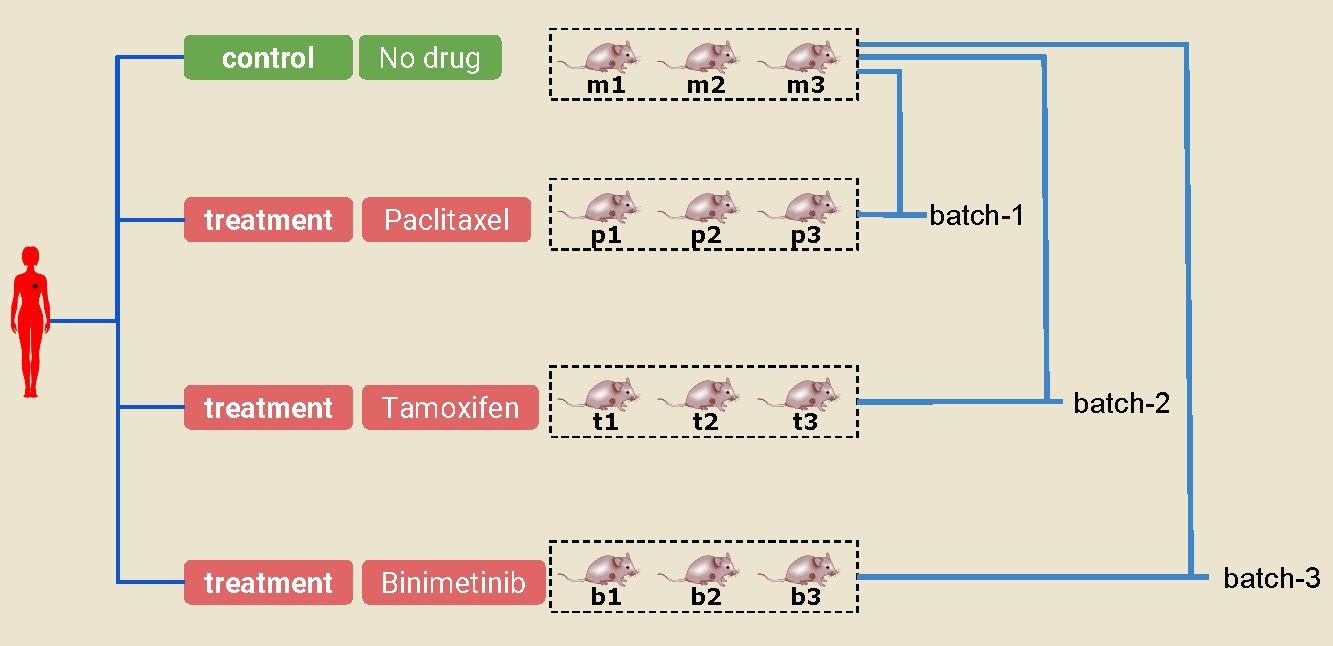
\includegraphics[keepaspectratio=true,width=1\textwidth]{images/Xeva_batch_2.pdf}
    \caption{A PDX experiment. The text under each of the PDX/mouse (ie. m1, m2, p1, etc.) denotes the \textit{model.id} in \textbf{Xeva}. In this example, three PDXs are delclared as control (m1, m2, and m3). Similarly, in the treatment arm, 3 PDXs are given the drug paclitaxel (p1, p2, and p3), 3 are given tamoxifen (t1, t2, and t3), and 3 are given binimetinib (b1, b2, b3). The PDXs in the control arm and one of the treatment arms together constitute a \textit{batch}. For example, control arm models (m1, m2, and m3) and treatment arm models (t1,t2, and t3) together create a batch called batch-2. } \label{fig:1}
\end{figure}

A \textbf{Xeva} object binds together all individual experiments, batch information, and molecular data into one single class called XevaSet.


\section{Data Access}
As mentioned earlier, \textbf{Xeva} stores metadata for each individual PDX model.
We can retrieve the meta-information about each PDX, such as number of models and tissue type, using:
\begin{knitrout}
\definecolor{shadecolor}{rgb}{0.969, 0.969, 0.969}\color{fgcolor}\begin{kframe}
\begin{alltt}
\hlstd{brca.mod} \hlkwb{<-} \hlkwd{modelInfo}\hlstd{(brca)}
\hlkwd{dim}\hlstd{(brca.mod)}
\end{alltt}
\begin{verbatim}
## [1] 849   5
\end{verbatim}
\begin{alltt}
\hlstd{brca.mod[}\hlnum{1}\hlopt{:}\hlnum{4}\hlstd{, ]}
\end{alltt}
\begin{verbatim}
##                model.id tissue   tissue.name patient.id        drug
## X.1004.BG98 X.1004.BG98   BRCA Breast Cancer     X-1004      BGJ398
## X.1004.biib X.1004.biib   BRCA Breast Cancer     X-1004 binimetinib
## X.1004.BK20 X.1004.BK20   BRCA Breast Cancer     X-1004      BKM120
## X.1004.BY19 X.1004.BY19   BRCA Breast Cancer     X-1004      BYL719
\end{verbatim}
\end{kframe}
\end{knitrout}
The output shows that the \textit{brca} dataset contains 849 PDX models.
We can also see the time vs. tumor volume data for a model using:

\begin{knitrout}
\definecolor{shadecolor}{rgb}{0.969, 0.969, 0.969}\color{fgcolor}\begin{kframe}
\begin{alltt}
\hlstd{model.data} \hlkwb{<-} \hlkwd{getExperiment}\hlstd{(brca,} \hlkwc{model.id} \hlstd{=} \hlstr{"X.1004.BG98"}\hlstd{)}
\hlkwd{head}\hlstd{(model.data)}
\end{alltt}
\begin{verbatim}
##      model.id drug.join.name time volume body.weight volume.normal
## 1 X.1004.BG98         BGJ398    0  199.7        28.2     0.0000000
## 2 X.1004.BG98         BGJ398    2  181.9        28.0    -0.0891337
## 3 X.1004.BG98         BGJ398    5  172.7        28.4    -0.1352028
## 4 X.1004.BG98         BGJ398    9  129.6        27.2    -0.3510265
## 5 X.1004.BG98         BGJ398   12   91.3        26.7    -0.5428142
## 6 X.1004.BG98         BGJ398   16  117.1        26.2    -0.4136204
\end{verbatim}
\end{kframe}
\end{knitrout}

Similarly, for \textbf{batch} names, we can obtain all predefined batch names using:

\begin{knitrout}
\definecolor{shadecolor}{rgb}{0.969, 0.969, 0.969}\color{fgcolor}\begin{kframe}
\begin{alltt}
\hlstd{batch.name} \hlkwb{<-} \hlkwd{batchInfo}\hlstd{(brca)}
\hlstd{batch.name[}\hlnum{1}\hlopt{:}\hlnum{4}\hlstd{]}
\end{alltt}
\begin{verbatim}
## [1] "X-1004.BGJ398"      "X-1004.binimetinib" "X-1004.BKM120"     
## [4] "X-1004.BYL719"
\end{verbatim}
\end{kframe}
\end{knitrout}

The information about a \textbf{batch} can be shown using:
\begin{knitrout}
\definecolor{shadecolor}{rgb}{0.969, 0.969, 0.969}\color{fgcolor}\begin{kframe}
\begin{alltt}
\hlkwd{batchInfo}\hlstd{(brca,} \hlkwc{batch} \hlstd{=} \hlstr{"X-1004.binimetinib"}\hlstd{)}
\end{alltt}
\begin{verbatim}
## $`X-1004.binimetinib`
## name = X-1004.binimetinib
## control = X.1004.uned
## treatment = X.1004.biib
## drug = binimetinib
## patient.id = X-1004
\end{verbatim}
\end{kframe}
\end{knitrout}
Here, for the batch named \textit{X-1004.binimetinib}, we can see that the control sample is \textit{X.1004.uned} and the treatment sample is \textit{X.1004.biib}.



\section{Visualizing PDX Growth Curve}

Xeva provides a function to plot time vs. tumor volume data for individual models as well as for individual batches. These data can be plotted by using the name of the batch:
\begin{knitrout}
\definecolor{shadecolor}{rgb}{0.969, 0.969, 0.969}\color{fgcolor}\begin{kframe}
\begin{alltt}
\hlkwd{plotPDX}\hlstd{(brca,} \hlkwc{batch} \hlstd{=} \hlstr{"X-4567.BKM120"}\hlstd{)}
\end{alltt}
\end{kframe}\begin{figure}
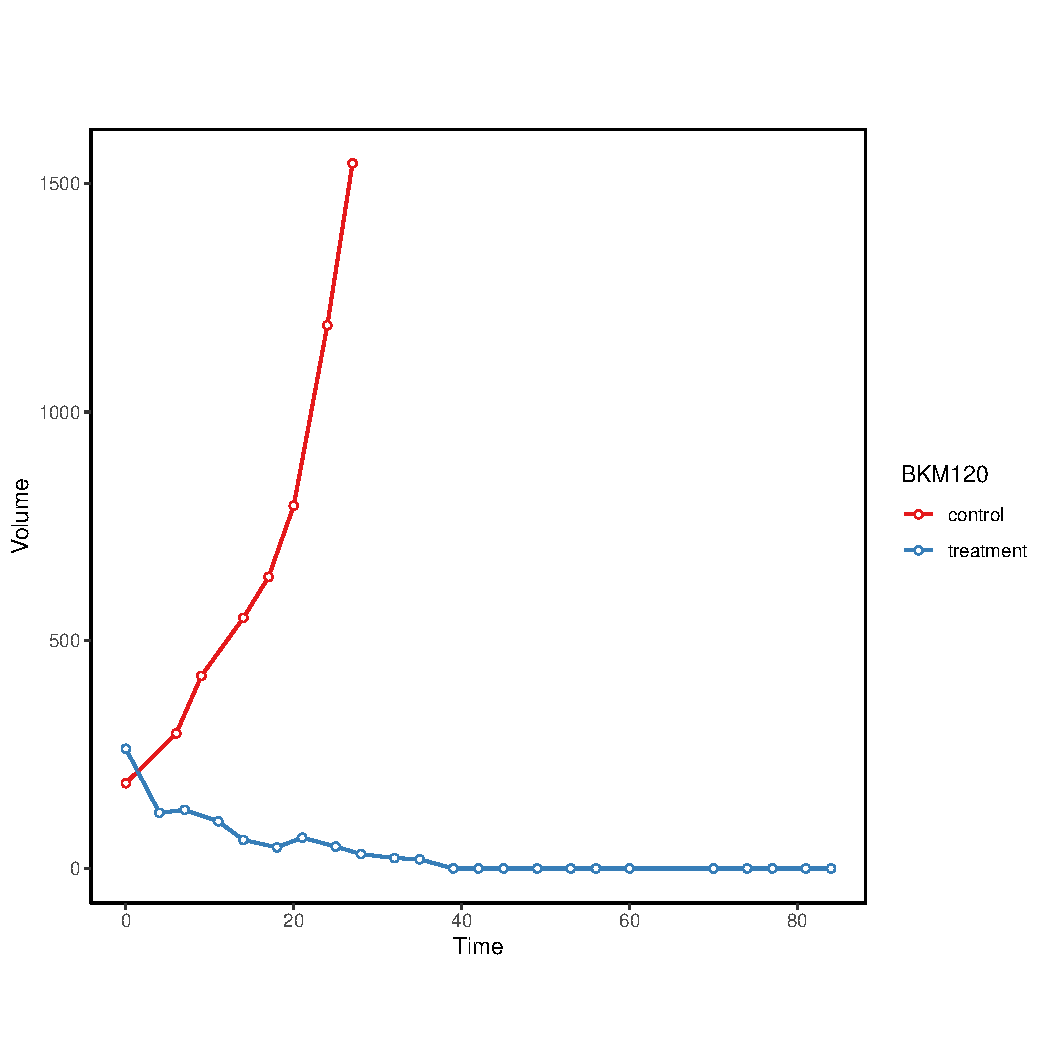
\includegraphics[width=4in]{figure/plot1-1} \caption[Tumor growth curves for a batch of control and treated PDXs]{Tumor growth curves for a batch of control and treated PDXs}\label{fig:plot1}
\end{figure}

\end{knitrout}


You can choose to see different aspects of this visualization. For example, we can plot normalized volume; we can also change the colors of the lines:
\begin{knitrout}
\definecolor{shadecolor}{rgb}{0.969, 0.969, 0.969}\color{fgcolor}\begin{kframe}
\begin{alltt}
\hlkwd{plotPDX}\hlstd{(brca,} \hlkwc{batch} \hlstd{=} \hlstr{"X-4567.BKM120"}\hlstd{,} \hlkwc{vol.normal} \hlstd{=} \hlnum{TRUE}\hlstd{,} \hlkwc{control.col} \hlstd{=} \hlstr{"#a6611a"}\hlstd{,}
        \hlkwc{treatment.col} \hlstd{=} \hlstr{"#018571"}\hlstd{,} \hlkwc{major.line.size} \hlstd{=} \hlnum{1}\hlstd{,} \hlkwc{max.time} \hlstd{=} \hlnum{40}\hlstd{)}
\end{alltt}
\end{kframe}\begin{figure}
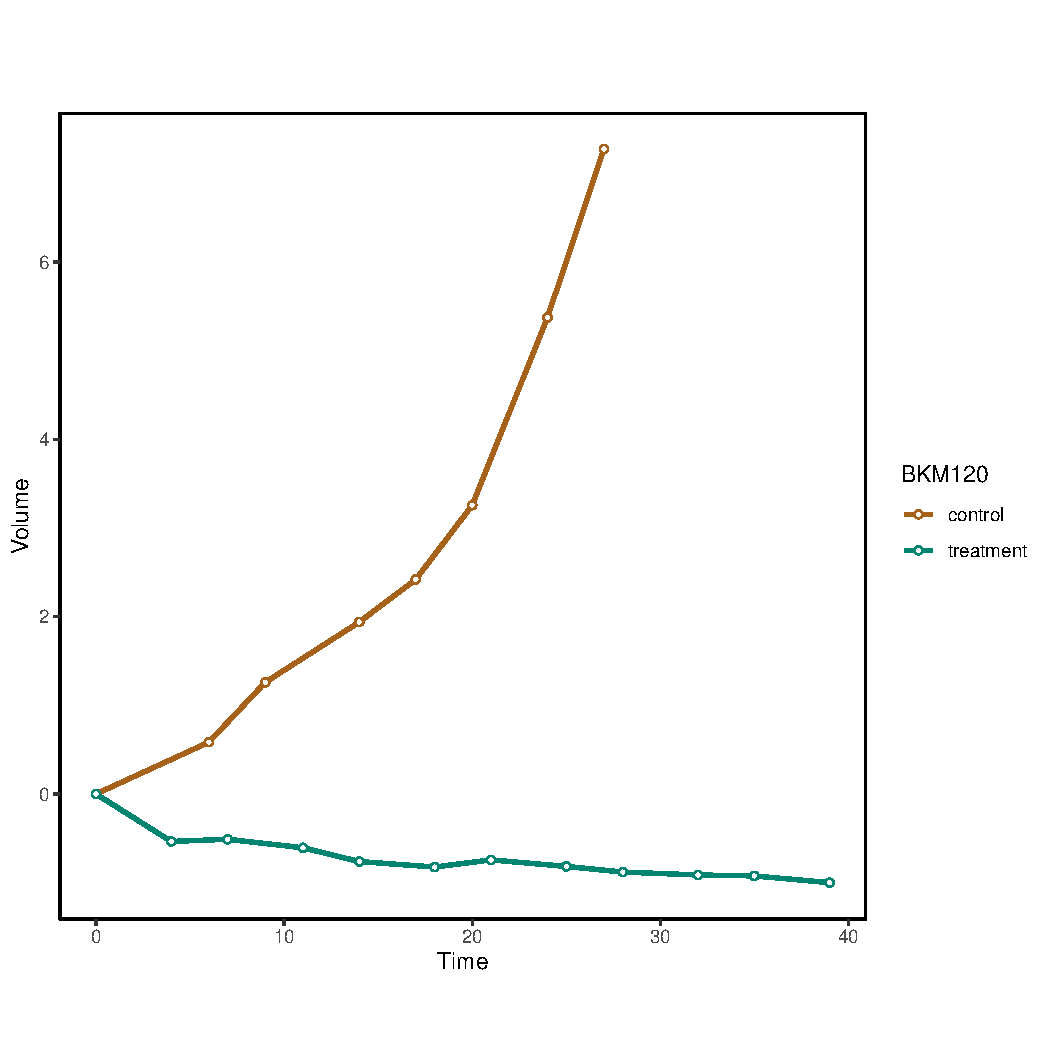
\includegraphics[width=4in]{figure/pdxplot2-1} \caption[Tumor growth curves for a batch of control and treated PDXs]{Tumor growth curves for a batch of control and treated PDXs. Here, the volume is normalized and plots are truncated at 40 days}\label{fig:pdxplot2}
\end{figure}

\end{knitrout}


Data can also be visualized at the patient level by specifying \texttt{patient.id}:
%%##X-2344, X-1004, X-3078 and X-5975
\begin{knitrout}
\definecolor{shadecolor}{rgb}{0.969, 0.969, 0.969}\color{fgcolor}\begin{kframe}
\begin{alltt}
\hlkwd{plotPDX}\hlstd{(brca,} \hlkwc{patient.id}\hlstd{=}\hlstr{"X-3078"}\hlstd{,} \hlkwc{drug}\hlstd{=}\hlstr{"paclitaxel"}\hlstd{,}\hlkwc{control.name} \hlstd{=} \hlstr{"untreated"}\hlstd{)}
\end{alltt}
\end{kframe}\begin{figure}
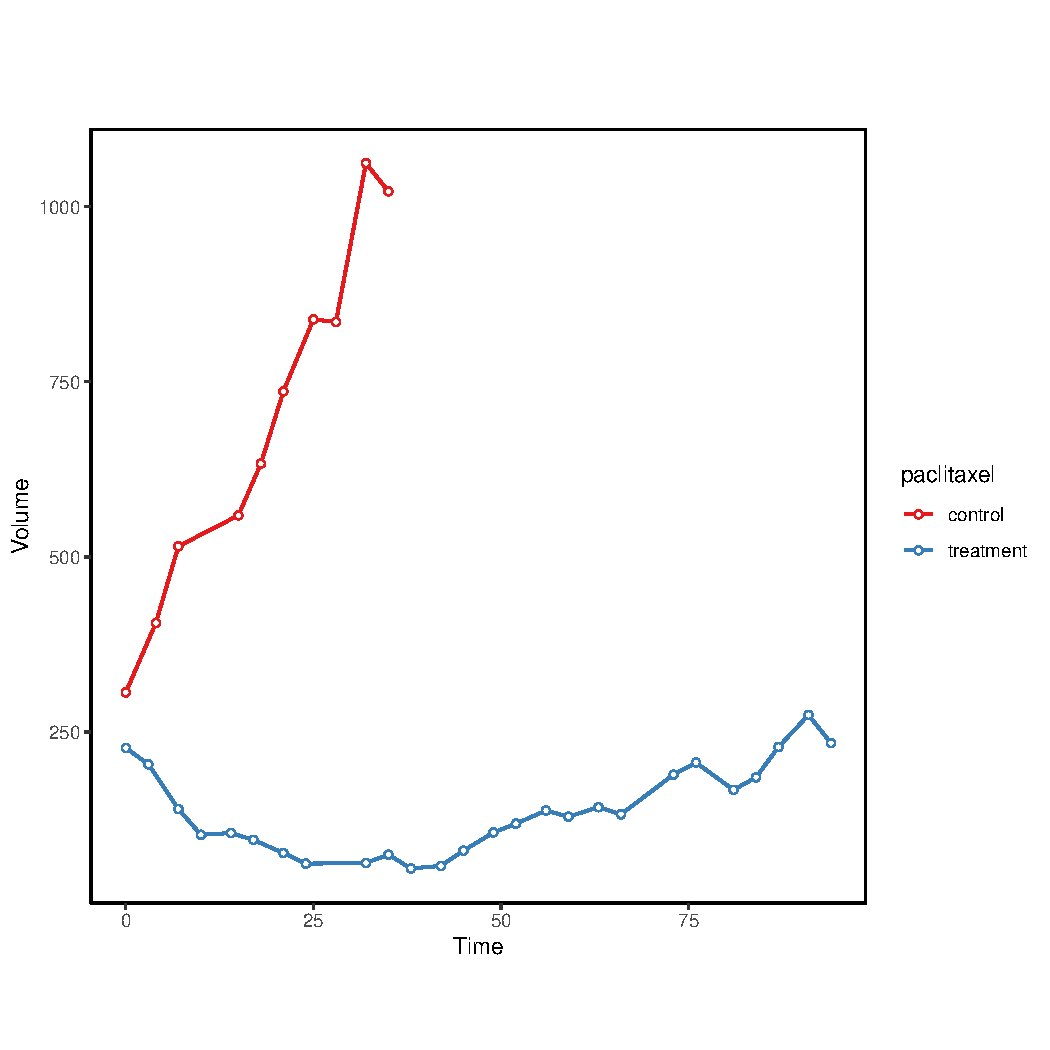
\includegraphics[width=4in]{figure/pdxplot3-1} \caption[Tumor growth curves for a batch of control and treated PDXs generated using patient ID and drug name]{Tumor growth curves for a batch of control and treated PDXs generated using patient ID and drug name}\label{fig:pdxplot3}
\end{figure}

\end{knitrout}



\section{Replicate-based PDX experiments}
Xeva can also handle replicate-based experiment design. The datasets included in the package also contain replicate-based PDX experiments. To plot replicate-based data:
\begin{knitrout}
\definecolor{shadecolor}{rgb}{0.969, 0.969, 0.969}\color{fgcolor}\begin{kframe}
\begin{alltt}
\hlkwd{data}\hlstd{(}\hlstr{"repdx"}\hlstd{)}
\hlkwd{plotPDX}\hlstd{(repdx,} \hlkwc{vol.normal} \hlstd{=} \hlnum{TRUE}\hlstd{,} \hlkwc{batch} \hlstd{=} \hlstr{"P1"}\hlstd{)}
\end{alltt}
\end{kframe}\begin{figure}
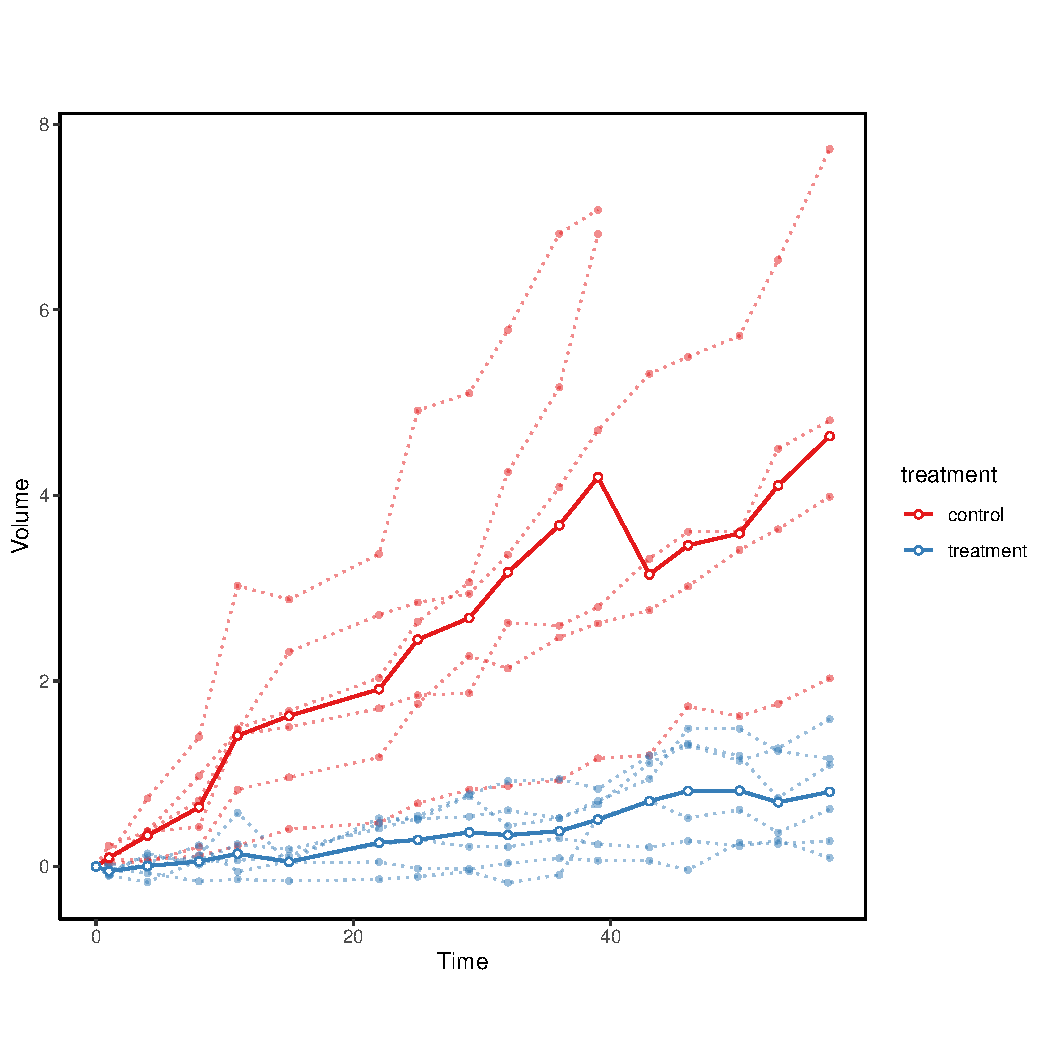
\includegraphics[width=4in]{figure/repplot1-1} \caption[Tumor growth curves for a batch of control and treated PDXs with replicates]{Tumor growth curves for a batch of control and treated PDXs with replicates}\label{fig:repplot1}
\end{figure}

\end{knitrout}

\begin{knitrout}
\definecolor{shadecolor}{rgb}{0.969, 0.969, 0.969}\color{fgcolor}\begin{kframe}
\begin{alltt}
\hlkwd{plotPDX}\hlstd{(repdx,} \hlkwc{batch} \hlstd{=} \hlstr{"P3"}\hlstd{,} \hlkwc{SE.plot} \hlstd{=} \hlstr{"errorbar"}\hlstd{)}
\end{alltt}
\end{kframe}\begin{figure}
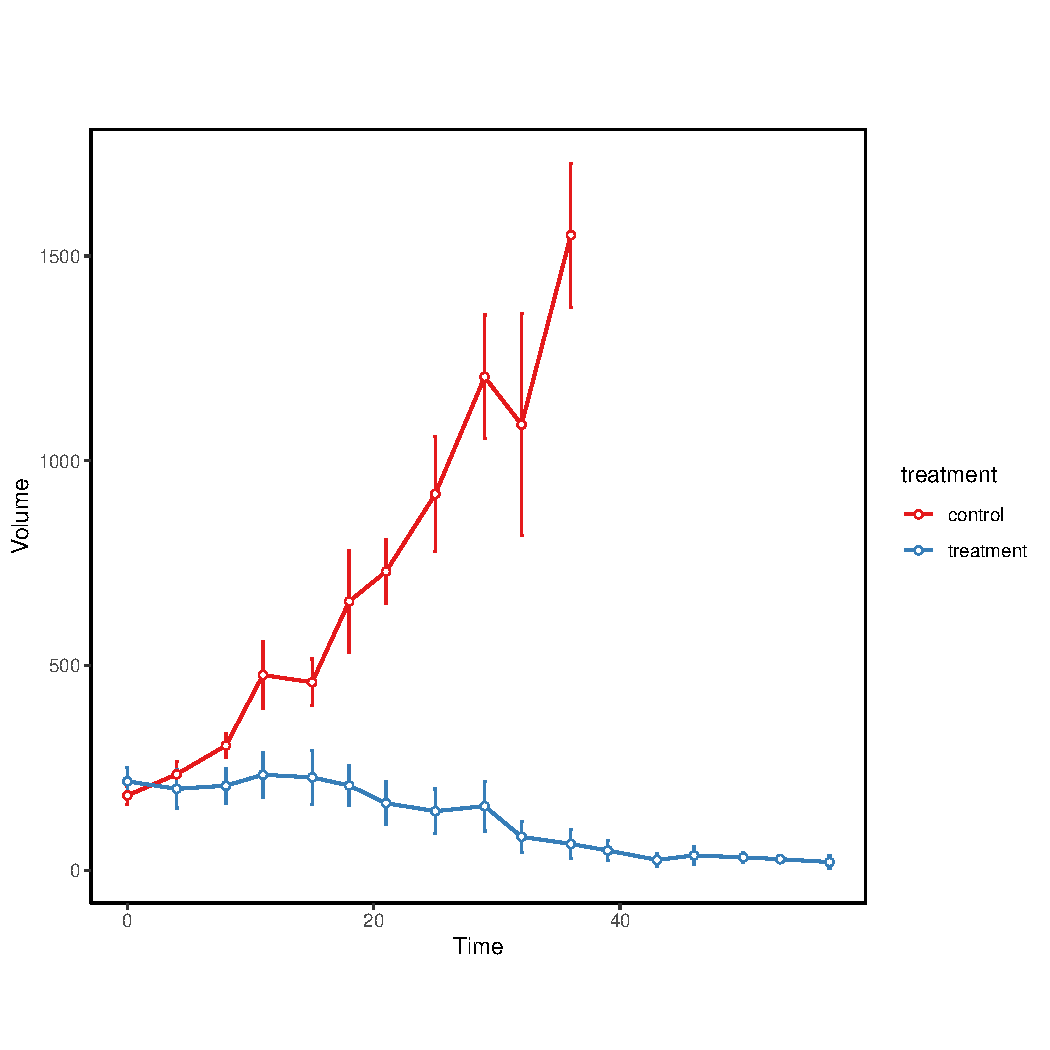
\includegraphics[width=4in]{figure/repplot2-1} \caption[Errorbar visualization for tumor growth curves of a PDX batch]{Errorbar visualization for tumor growth curves of a PDX batch}\label{fig:repplot2}
\end{figure}

\end{knitrout}

\begin{knitrout}
\definecolor{shadecolor}{rgb}{0.969, 0.969, 0.969}\color{fgcolor}\begin{kframe}
\begin{alltt}
\hlkwd{plotPDX}\hlstd{(repdx,} \hlkwc{batch} \hlstd{=} \hlstr{"P4"}\hlstd{,} \hlkwc{vol.normal} \hlstd{=} \hlnum{TRUE}\hlstd{,}  \hlkwc{SE.plot} \hlstd{=} \hlstr{"ribbon"}\hlstd{)}
\end{alltt}
\end{kframe}\begin{figure}
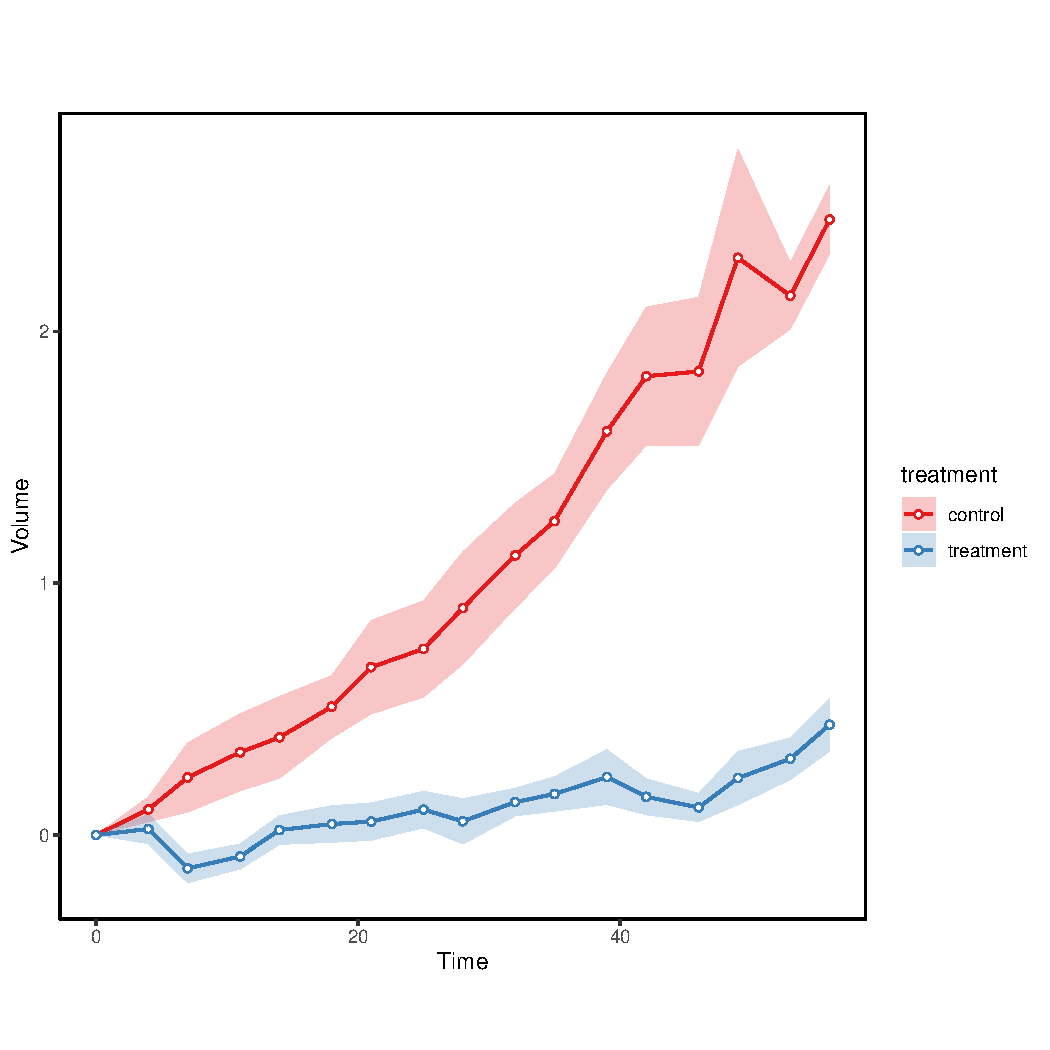
\includegraphics[width=4in]{figure/repplot3-1} \caption[Ribbon visualization for tumor growth curves of a PDX batch]{Ribbon visualization for tumor growth curves of a PDX batch}\label{fig:repplot3}
\end{figure}

\end{knitrout}


\section{PDX Model Drug Response}  \label{response}

%%%%%%%%%%%%%%%%%%%
\subsection{PDX response calculation}
In Xeva, we have implemented several response metrics.
There are two kinds of response metrics available:

\begin{enumerate}
	\item Model response: This type of response is computed for any individual PDX model.
	Examples include how fast a PDX model is growing or how long the PDX survives.
	Such response does not take into account the control PDX as it is computed for an individual PDX model.
	In this category the following metrics can be computed:
    \begin{enumerate}
    	\item mRECIST and associated metrics best.response (BR), best.average.response (BAR).
    	mRECIST divides response into 4 categories  \cite{MerXeva}.
      	\begin{itemize}
      	\item complete response (CR): BR < -95\% and BAR < -40\%
      	\item partial response (PR): BR < -50\% and BAR < -20\%
      	\item stable disease (SD): BR < 35\% and BAR < 30\%
      	\item progressive disease (PD): not otherwise categorized
      	\end{itemize}

      \item slope is defined as angle of PDX volume curve.
      \item AUC (area under the curve) represents area covered by PDX curve per day (AUC divided by time).
    \end{enumerate}

    \item Batch response: This type of response is computed by taking into account models in control and treatment group. In this category the following metrics can be computed:
    \begin{enumerate}
    \item Angle between treatment and control PDXs
    \item abc (area between the curves) is computed as difference in AUC of control and treatment.
    \item TGI (tumor growth inhibition)
    \item lmm (linear mix model)
    \item bmRECIST (batch level mRECIST, computed separately for control and treatment arm)
    \end{enumerate}
\end{enumerate}


\begin{tcolorbox}[fonttitle=\sffamily\bfseries\large,
%colframe=red!75!black,
title=Note: mRECIST and bmRECIST]
The response metric \textbf{mRECIST} can only be computed for a single PDX model at a time.
Moreover for a treatment model it doesn't take into account corresponding control models.
Response for all individual models in a batch can be extracted using \textit{summarizeResponse} function (also see \ref{visRes}).
We have implemented \textbf{bmRECIST}  which is the mRECIST for a batch.
This is simply \textbf{mRECIST} computed on the average time-volume curve
(from multiple PDX models).
In this setting we compute \textbf{mRECIST} separately for treatment and control arm.
These ouputs are represented as \textit{mRECIST.control} and \textit{mRECIST.treatment}
in the sensitivity slot.
At present it is not possible to combine \textit{mRECIST.control} and \textit{mRECIST.treatment} in one single metric. However we are working on this and  will update the Xeva code in future with such metric.

\end{tcolorbox}

%%%%%%%%%%%%%%%%

In Xeva we have provided a unified function \textbf{\textcolor{red}{\hl{response}}}
to compute all different response metrics.
Functions for individual response metrics are also available for use (see documention of the package for details).
To compute mRECIST of a model:

\begin{knitrout}
\definecolor{shadecolor}{rgb}{0.969, 0.969, 0.969}\color{fgcolor}\begin{kframe}
\begin{alltt}
\hlkwd{response}\hlstd{(brca,} \hlkwc{model.id}\hlstd{=}\hlstr{"X.1004.BG98"}\hlstd{,} \hlkwc{res.measure}\hlstd{=}\hlstr{"mRECIST"}\hlstd{)}
\end{alltt}
\begin{verbatim}
## computing mRECIST for X.1004.BG98
## mRECIST = PR
## Best average response = -28.0754
## Best response = -54.2814
\end{verbatim}
\end{kframe}
\end{knitrout}

Similarly, TGI (a batch level response) can be computed as:
\begin{knitrout}
\definecolor{shadecolor}{rgb}{0.969, 0.969, 0.969}\color{fgcolor}\begin{kframe}
\begin{alltt}
\hlkwd{response}\hlstd{(brca,} \hlkwc{batch}\hlstd{=}\hlstr{"X-6047.paclitaxel"}\hlstd{,} \hlkwc{res.measure}\hlstd{=}\hlstr{"TGI"}\hlstd{)}
\end{alltt}
\begin{verbatim}
## computing TGI for batch X-6047.paclitaxel
## TGI = 10.404412
\end{verbatim}
\end{kframe}
\end{knitrout}


\subsection{Setting response for XevaSet} \label{setresponse}
In a newly created Xevaset, one has to compute the response for all models and
batches before using it for analysis. This can be done easily using the \textbf{\textcolor{red}{\hl{setResponse}}}  function.
In this example we are computing mRECIST for all models and getting an updated
XevaSet (which contains mRECIST values):

\begin{knitrout}
\definecolor{shadecolor}{rgb}{0.969, 0.969, 0.969}\color{fgcolor}\begin{kframe}
\begin{alltt}
\hlstd{brca}  \hlkwb{<-} \hlkwd{setResponse}\hlstd{(brca,} \hlkwc{res.measure} \hlstd{=} \hlstr{"mRECIST"}\hlstd{,} \hlkwc{verbose}\hlstd{=}\hlnum{FALSE}\hlstd{)}
\end{alltt}
\end{kframe}
\end{knitrout}

Next we update the object by computing the TGI as:
\begin{knitrout}
\definecolor{shadecolor}{rgb}{0.969, 0.969, 0.969}\color{fgcolor}\begin{kframe}
\begin{alltt}
\hlstd{brca}  \hlkwb{<-} \hlkwd{setResponse}\hlstd{(brca,} \hlkwc{res.measure} \hlstd{=} \hlstr{"TGI"}\hlstd{,} \hlkwc{verbose}\hlstd{=}\hlnum{FALSE}\hlstd{)}
\end{alltt}
\end{kframe}
\end{knitrout}


\subsection{Visualizing PDX response} \label{visRes}
Xeva can effectively summarize PDX drug response data.
To get \textbf{mRECIST} for all models in a single batch:
\begin{knitrout}
\definecolor{shadecolor}{rgb}{0.969, 0.969, 0.969}\color{fgcolor}\begin{kframe}
\begin{alltt}
\hlstd{r} \hlkwb{<-} \hlkwd{summarizeResponse}\hlstd{(brca,}\hlkwc{response.measure}\hlstd{=}\hlstr{"mRECIST"}\hlstd{,}\hlkwc{batch.id}\hlstd{=}\hlstr{"X-1004.BGJ398"}\hlstd{)}
\hlkwd{head}\hlstd{(r)}
\end{alltt}
\begin{verbatim}
##                model.id    batch.name      type mRECIST
## X.1004.uned X.1004.uned X-1004.BGJ398   control      PD
## X.1004.BG98 X.1004.BG98 X-1004.BGJ398 treatment      PR
\end{verbatim}
\end{kframe}
\end{knitrout}


Next we summarize the \textbf{mRECIST} values for the models in our dataset:
\begin{knitrout}
\definecolor{shadecolor}{rgb}{0.969, 0.969, 0.969}\color{fgcolor}\begin{kframe}
\begin{alltt}
\hlstd{brca.mr} \hlkwb{<-} \hlkwd{summarizeResponse}\hlstd{(brca,} \hlkwc{response.measure}\hlstd{=}\hlstr{"mRECIST"}\hlstd{,}
                             \hlkwc{group.by}\hlstd{=}\hlstr{"patient.id"}\hlstd{)}
\hlstd{brca.mr[}\hlnum{1}\hlopt{:}\hlnum{5}\hlstd{,} \hlnum{1}\hlopt{:}\hlnum{4}\hlstd{]}
\end{alltt}
\begin{verbatim}
##                 X-1004 X-1008 X-1286 X-1298
## BGJ398          "PR"   "SD"   "PD"   "SD"  
## binimetinib     "PD"   "SD"   "SD"   "PD"  
## BKM120          "SD"   "SD"   "SD"   "PR"  
## BYL719          "SD"   "PR"   "SD"   "PD"  
## BYL719 + LEE011 "PD"   "SD"   "SD"   "PD"
\end{verbatim}
\end{kframe}
\end{knitrout}

These \textbf{mRECIST} values can be visualized using:
\begin{knitrout}
\definecolor{shadecolor}{rgb}{0.969, 0.969, 0.969}\color{fgcolor}\begin{kframe}
\begin{alltt}
\hlkwd{plotmRECIST}\hlstd{(brca.mr,} \hlkwc{control.name}\hlstd{=}\hlstr{"untreated"}\hlstd{,} \hlkwc{row_fontsize}\hlstd{=}\hlnum{13}\hlstd{,} \hlkwc{col_fontsize}\hlstd{=}\hlnum{12}\hlstd{)}
\end{alltt}
\end{kframe}\begin{figure}
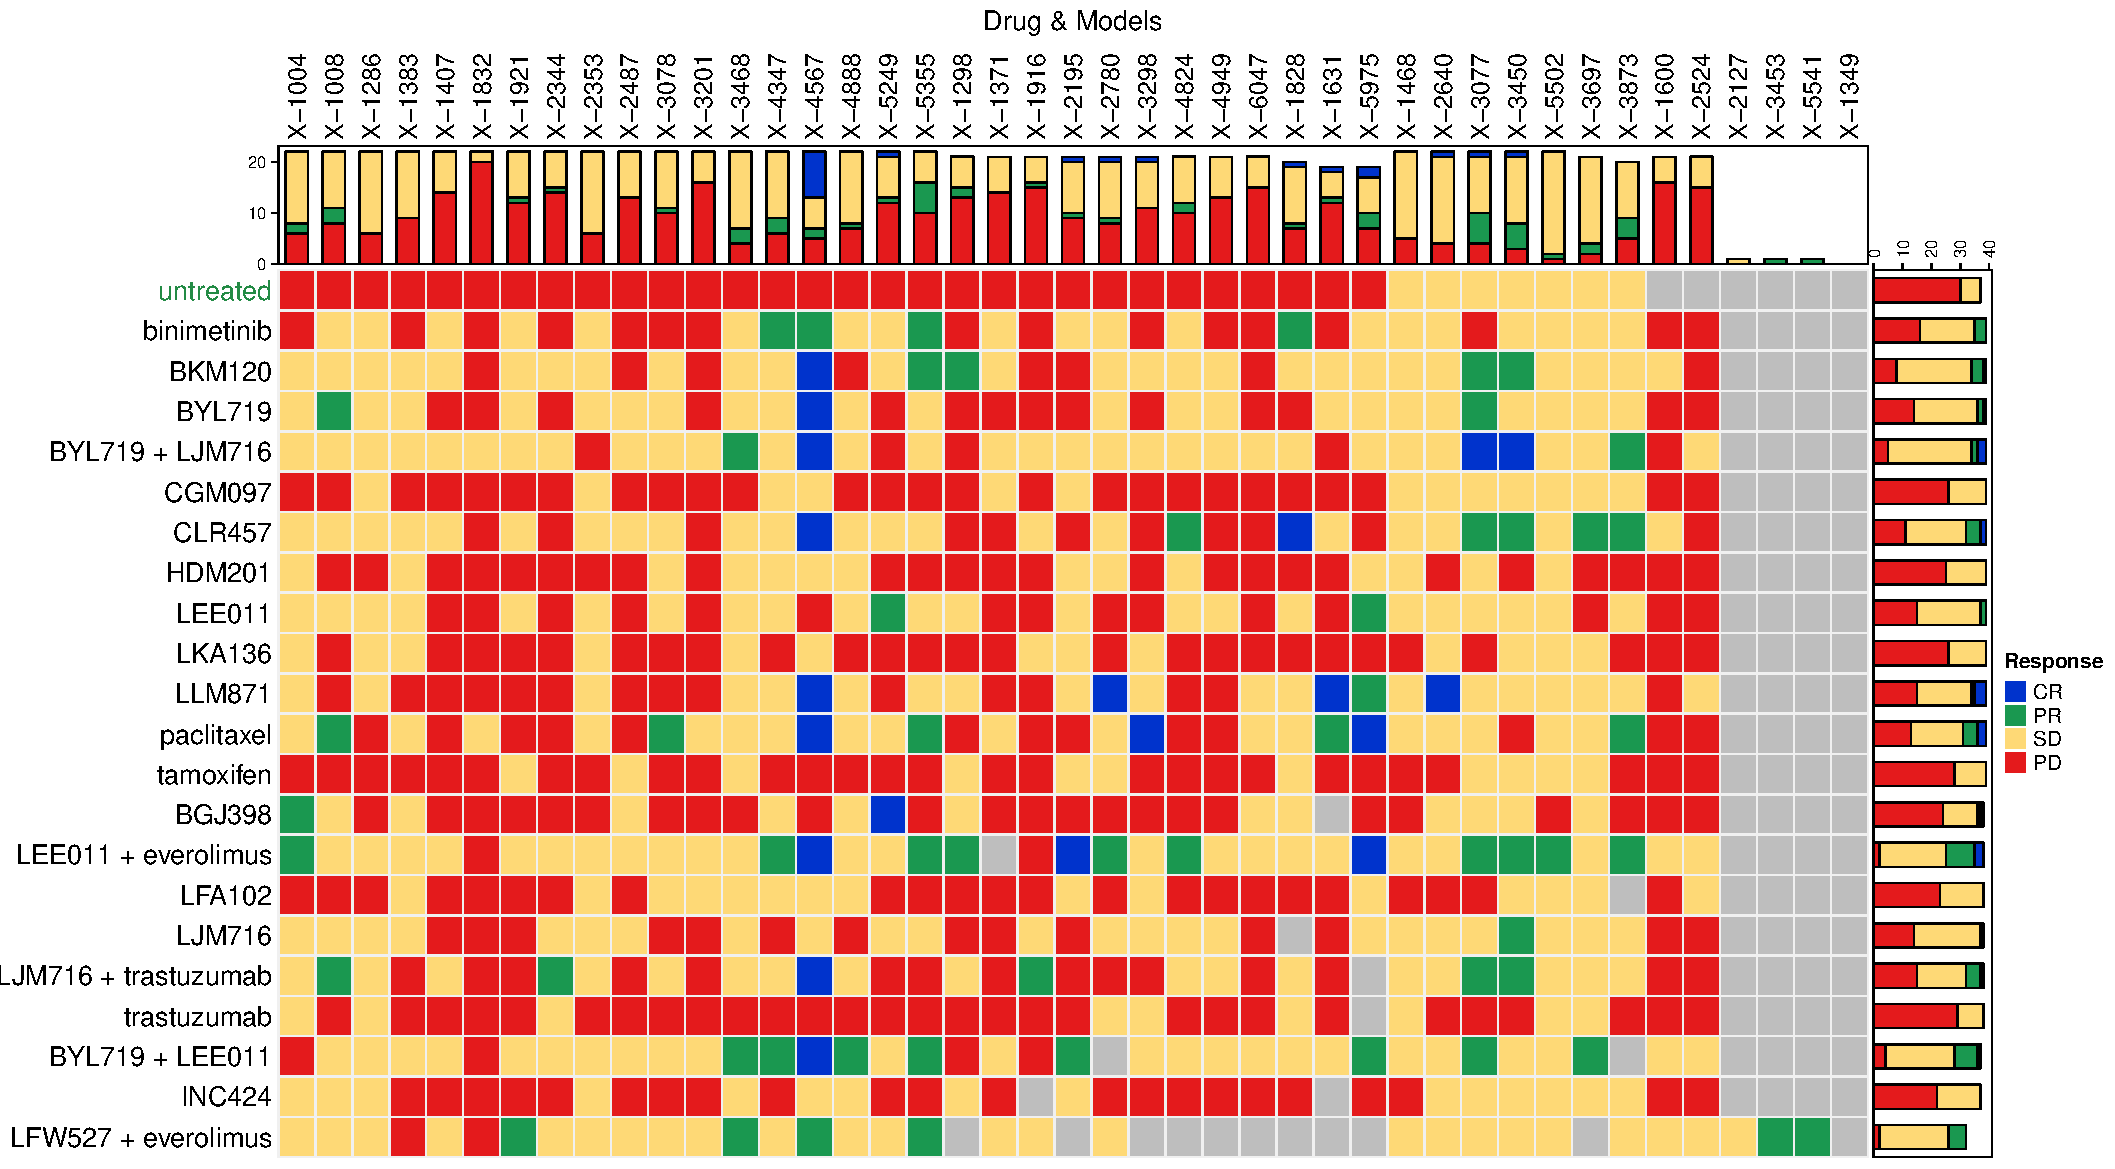
\includegraphics[width=\maxwidth]{figure/mR_BRCA-1} \caption[mRECIST plot for PDXE breast cancer data]{mRECIST plot for PDXE breast cancer data}\label{fig:mR_BRCA}
\end{figure}

\end{knitrout}


Waterfall plots are also commonly used to visualize PDX drug response data.
Xeva provides a function to visualize and color waterfall plots:
\begin{knitrout}
\definecolor{shadecolor}{rgb}{0.969, 0.969, 0.969}\color{fgcolor}\begin{kframe}
\begin{alltt}
\hlkwd{waterfall}\hlstd{(brca,} \hlkwc{drug}\hlstd{=}\hlstr{"binimetinib"}\hlstd{,} \hlkwc{res.measure}\hlstd{=}\hlstr{"best.average.response"}\hlstd{)}
\end{alltt}
\end{kframe}\begin{figure}
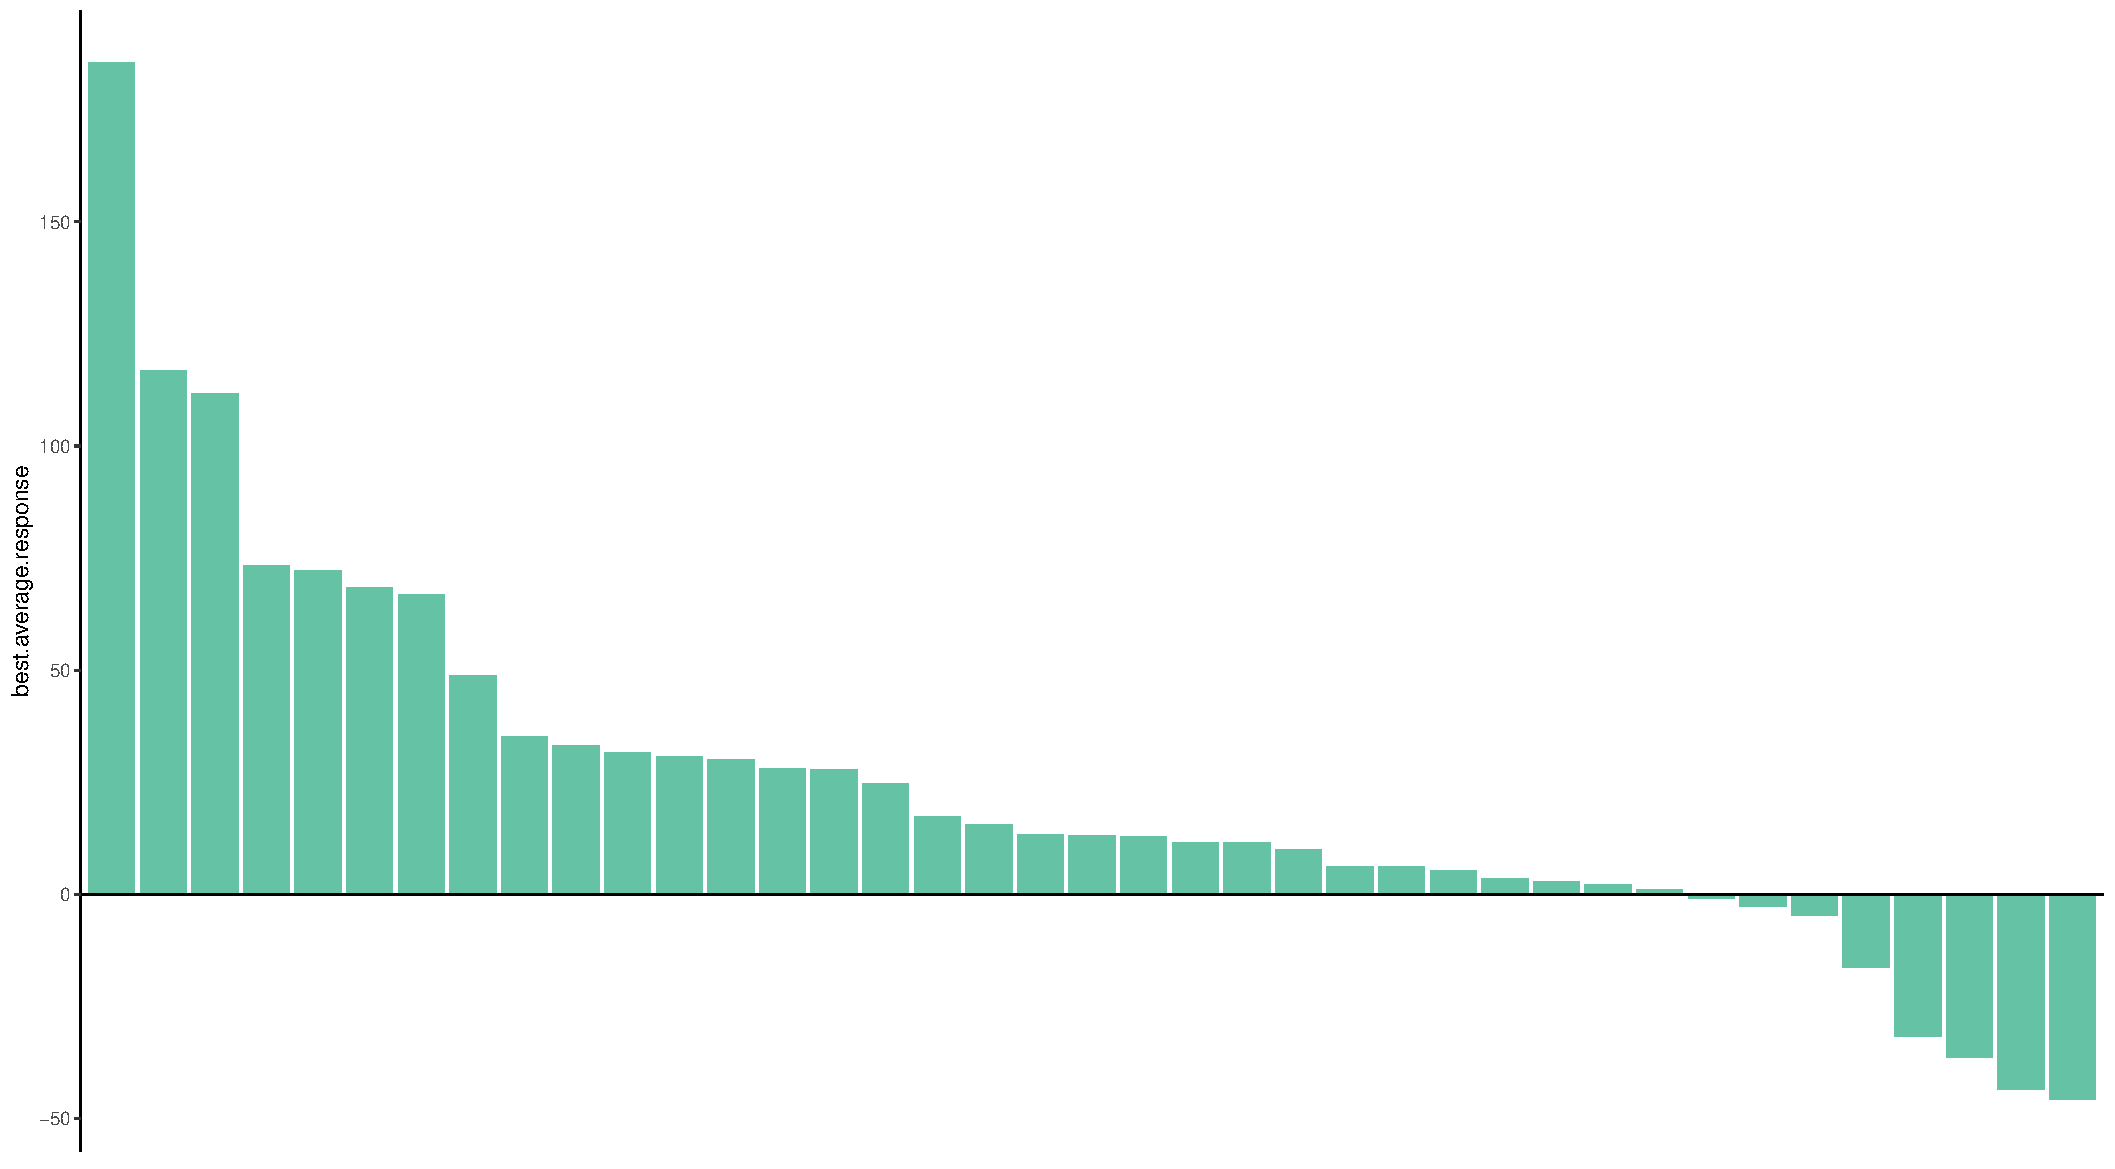
\includegraphics[width=\maxwidth]{figure/waterFall1-1} \caption[Waterfall plot for binimetinib drug response in PDXs]{Waterfall plot for binimetinib drug response in PDXs}\label{fig:waterFall1}
\end{figure}

\end{knitrout}


It is useful to color the bars of your waterfall plot by genomic properties.
If the color type information is available in `modelInfo`, colored bars can be directly be plotted by specifying name of the column for `type` parameter.
Otherwise one can extract a data.frame of response and add a column for `type` and visualize the waterfall plot.
Here we create a waterfall plot for drug BYL719 and color it based on the mutation status of the CDK13 gene:
\begin{knitrout}
\definecolor{shadecolor}{rgb}{0.969, 0.969, 0.969}\color{fgcolor}\begin{kframe}
\begin{alltt}
\hlkwd{data}\hlstd{(brca)}

\hlcom{## extract mutation information}
\hlstd{mut} \hlkwb{<-} \hlkwd{summarizeData}\hlstd{(brca,} \hlkwc{drug} \hlstd{=} \hlstr{"BYL719"}\hlstd{,} \hlkwc{mDataType}\hlstd{=}\hlstr{"mutation"}\hlstd{)}
\hlstd{model.type} \hlkwb{<-} \hlstd{Biobase}\hlopt{::}\hlkwd{exprs}\hlstd{(mut)[}\hlstr{"CDK13"}\hlstd{, ]}

\hlcom{## extract data.frame of response}
\hlstd{df} \hlkwb{<-} \hlkwd{summarizeResponse}\hlstd{(brca,} \hlkwc{response.measure} \hlstd{=} \hlstr{"best.average.response"}\hlstd{,}
                        \hlkwc{return.type} \hlstd{=} \hlstr{"data.frame"}\hlstd{)}
\hlstd{df} \hlkwb{<-} \hlstd{df[df}\hlopt{$}\hlstd{drug} \hlopt{==} \hlstr{"BYL719"}\hlstd{, ]}

\hlcom{## add values to data.frame}
\hlstd{df}\hlopt{$}\hlstd{CDK13} \hlkwb{<-} \hlstd{model.type[df}\hlopt{$}\hlstd{patient.id]}
\hlcom{## now plot the data}

\hlkwd{waterfall}\hlstd{(df,} \hlkwc{x}\hlstd{=}\hlstr{"model.id"}\hlstd{,} \hlkwc{y}\hlstd{=}\hlstr{"best.average.response"}\hlstd{,} \hlkwc{type}\hlstd{=}\hlstr{"CDK13"}\hlstd{)}
\end{alltt}
\end{kframe}\begin{figure}
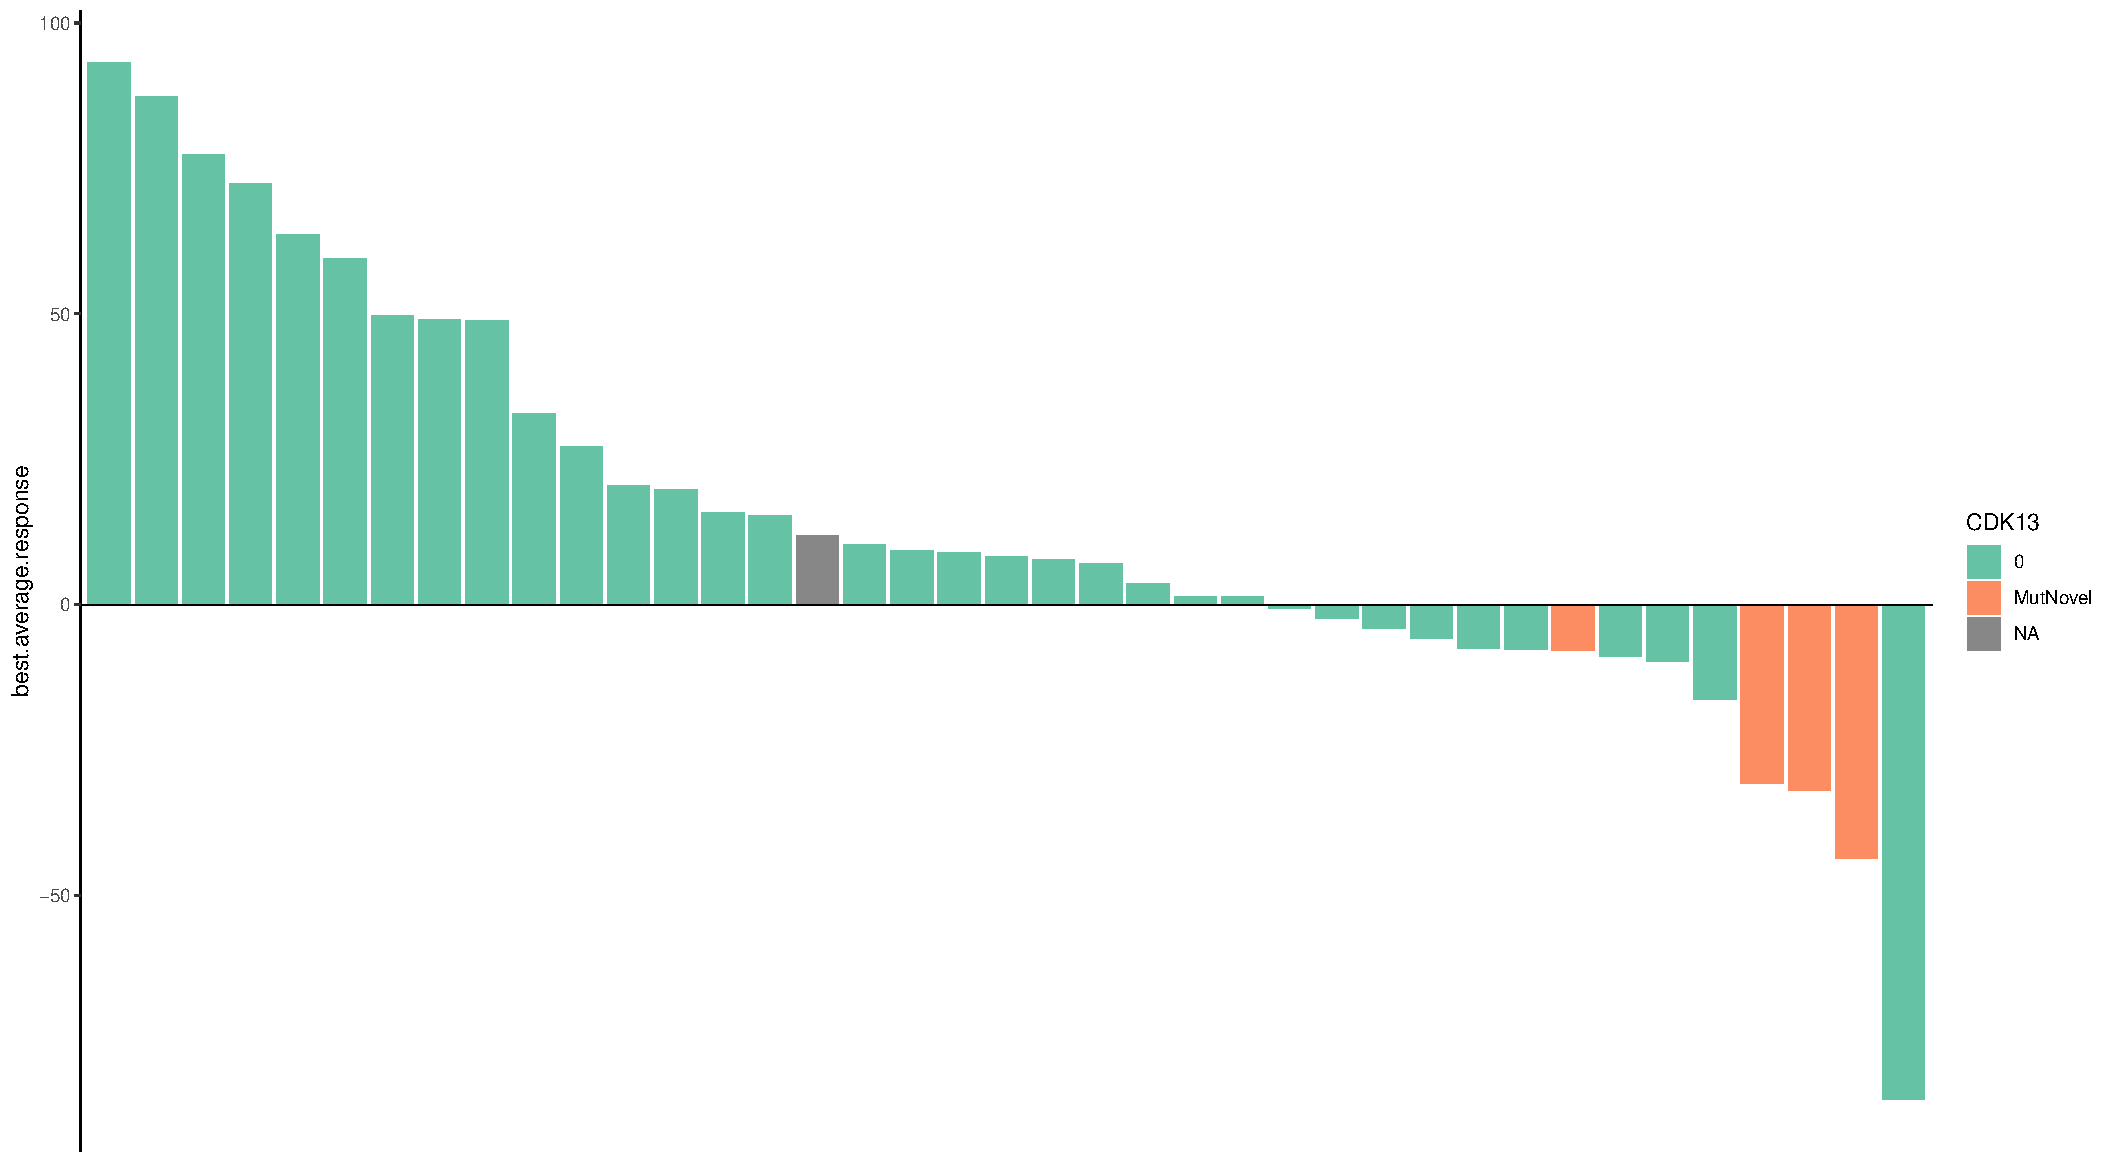
\includegraphics[width=\maxwidth]{figure/waterFall2-1} \caption[Waterfall plot for BYL719 drug response in PDXs]{Waterfall plot for BYL719 drug response in PDXs}\label{fig:waterFall2}
\end{figure}

\end{knitrout}

%%%%%%%%%%%%%%%%%%%%%%%%%%%%%%%%%%%%%%%%%
In Xeva we have implemented difference matrix to compute PDX response.
The Xeva function \textbf{\textcolor{red}{\hl{response}}} provides a unified interface for this purpose.
In the example below we compute the angle between treatment and control PDXs

\begin{knitrout}
\definecolor{shadecolor}{rgb}{0.969, 0.969, 0.969}\color{fgcolor}\begin{kframe}
\begin{alltt}
\hlkwd{data}\hlstd{(}\hlstr{"repdx"}\hlstd{)}
\hlkwd{response}\hlstd{(repdx,} \hlkwc{batch}\hlstd{=}\hlstr{"P1"}\hlstd{,} \hlkwc{res.measure}\hlstd{=}\hlstr{"angle"}\hlstd{)}
\end{alltt}
\begin{verbatim}
## computing angle for batch P1
## angle = 3.829701
## control = 4.651435
## treatment = 0.821733
\end{verbatim}
\end{kframe}
\end{knitrout}

A function for linear mixed-effects model (lmm) has also been implemented.
\begin{knitrout}
\definecolor{shadecolor}{rgb}{0.969, 0.969, 0.969}\color{fgcolor}\begin{kframe}
\begin{alltt}
\hlkwd{data}\hlstd{(}\hlstr{"repdx"}\hlstd{)}
\hlkwd{response}\hlstd{(repdx,} \hlkwc{batch}\hlstd{=}\hlstr{"P1"}\hlstd{,} \hlkwc{res.measure}\hlstd{=}\hlstr{"lmm"}\hlstd{)}
\end{alltt}
\begin{verbatim}
## computing lmm for batch P1
## Linear mixed-effects model fit by REML
##   Data: data 
##   Log-restricted-likelihood: 3.184927
##   Fixed: volume ~ time * exp.type 
##            (Intercept)                   time      exp.typetreatment 
##             5.32592390             0.03091321            -0.28718018 
## time:exp.typetreatment 
##            -0.01983870 
## 
## Random effects:
##  Formula: ~1 | model.id
##         (Intercept)  Residual
## StdDev:   0.3802407 0.1975011
## 
## Number of Observations: 194
## Number of Groups: 12
\end{verbatim}
\end{kframe}
\end{knitrout}



\section{Gene-drug association}
The main aim of the pharmacogenomic experiments is to find biomarkers for drug response prediction.
The Xeva package provides the \textbf{\textcolor{red}{drugSensitivitySig}} function to compute the univariate association between PDX's molecular data (such as gene expression) and response to a drug (gene-drug association). In the example bellow, we are computing the association between gene expression (RNASeq)
and slope of the PDXs for the drug `tamoxifen` using linear regression (lm).

\begin{knitrout}
\definecolor{shadecolor}{rgb}{0.969, 0.969, 0.969}\color{fgcolor}\begin{kframe}
\begin{alltt}
\hlkwd{data}\hlstd{(brca)}
\hlkwd{drugSensitivitySig}\hlstd{(}\hlkwc{object}\hlstd{=brca,} \hlkwc{drug}\hlstd{=}\hlstr{"tamoxifen"}\hlstd{,} \hlkwc{mDataType}\hlstd{=}\hlstr{"RNASeq"}\hlstd{,}
                   \hlkwc{features}\hlstd{=}\hlkwd{c}\hlstd{(}\hlnum{1}\hlstd{,}\hlnum{2}\hlstd{,}\hlnum{3}\hlstd{,}\hlnum{4}\hlstd{,}\hlnum{5}\hlstd{),} \hlkwc{sensitivity.measure}\hlstd{=}\hlstr{"slope"}\hlstd{,} \hlkwc{fit}\hlstd{=}\hlstr{"lm"}\hlstd{)}
\end{alltt}
\begin{verbatim}
## Running for 38 samples with non NA sensitivity.measure
## Running for 38 samples with non NA sensitivity.measure and 5 features
##   feature      drug    estimate        se  n       tstat       fstat    pvalue
## 1  PIK3R6 tamoxifen  0.12174756 0.1654268 38  0.73596007 0.541637222 0.4665236
## 2   FGFR1 tamoxifen -0.16019355 0.1645143 38 -0.97373653 0.948162830 0.3366852
## 3   NTRK2 tamoxifen  0.16560706 0.1643653 38  1.00755487 1.015166810 0.3203927
## 4    AKT1 tamoxifen  0.00996873 0.1666584 38  0.05981535 0.003577876 0.9526335
## 5   FGFR4 tamoxifen  0.07953256 0.1661387 38  0.47871178 0.229164971 0.6350385
##   df       fdr
## 1 36 0.7775393
## 2 36 0.7775393
## 3 36 0.7775393
## 4 36 0.9526335
## 5 36 0.7937981
\end{verbatim}
\end{kframe}
\end{knitrout}

In this above example we took only 5 features (genes), however this can be
extended for any number of genes. For larger analyses, this function also provides
out of box parallel computation. Users can set the number of cores using the parameter
\textbf{\textcolor{red}{nthread}} in the function.

Users can choose different sensitivity measures of the PDX response for the
association analysis by setting the parameter \textbf{\textcolor{red}{sensitivity.measure}}.
For example, below we use \textit{\textcolor{red}{best.average.response}} as
the PDX's response matrix in the association analysis:
\begin{knitrout}
\definecolor{shadecolor}{rgb}{0.969, 0.969, 0.969}\color{fgcolor}\begin{kframe}
\begin{alltt}
\hlkwd{data}\hlstd{(brca)}
\hlkwd{drugSensitivitySig}\hlstd{(}\hlkwc{object}\hlstd{=brca,} \hlkwc{drug}\hlstd{=}\hlstr{"tamoxifen"}\hlstd{,} \hlkwc{mDataType}\hlstd{=}\hlstr{"RNASeq"}\hlstd{,}
                   \hlkwc{features}\hlstd{=}\hlkwd{c}\hlstd{(}\hlnum{1}\hlstd{,}\hlnum{2}\hlstd{,}\hlnum{3}\hlstd{,}\hlnum{4}\hlstd{,}\hlnum{5}\hlstd{),}
                   \hlkwc{sensitivity.measure}\hlstd{=}\hlstr{"best.average.response"}\hlstd{,} \hlkwc{fit} \hlstd{=} \hlstr{"lm"}\hlstd{)}
\end{alltt}
\begin{verbatim}
## Running for 38 samples with non NA sensitivity.measure
## Running for 38 samples with non NA sensitivity.measure and 5 features
##   feature      drug    estimate        se  n      tstat     fstat    pvalue df
## 1  PIK3R6 tamoxifen  0.10155551 0.1658050 38  0.6124998 0.3751559 0.5440570 36
## 2   FGFR1 tamoxifen  0.25347267 0.1612238 38  1.5721794 2.4717480 0.1246577 36
## 3   NTRK2 tamoxifen  0.15268488 0.1647125 38  0.9269782 0.8592885 0.3601112 36
## 4    AKT1 tamoxifen -0.19722241 0.1633931 38 -1.2070422 1.4569510 0.2352874 36
## 5   FGFR4 tamoxifen -0.06903067 0.1662691 38 -0.4151744 0.1723698 0.6804783 36
##         fdr
## 1 0.6800713
## 2 0.5882184
## 3 0.6001853
## 4 0.5882184
## 5 0.6804783
\end{verbatim}
\end{kframe}
\end{knitrout}


For the drug-gene association analysis, users can also choose a different method
of association calculation (such as concordance index, Pearson or Spearman
correlation) by setting the parameter \textit{\textcolor{red}{fit}}.
\begin{knitrout}
\definecolor{shadecolor}{rgb}{0.969, 0.969, 0.969}\color{fgcolor}\begin{kframe}
\begin{alltt}
\hlkwd{data}\hlstd{(brca)}
\hlkwd{drugSensitivitySig}\hlstd{(}\hlkwc{object}\hlstd{=brca,} \hlkwc{drug}\hlstd{=}\hlstr{"tamoxifen"}\hlstd{,} \hlkwc{mDataType}\hlstd{=}\hlstr{"RNASeq"}\hlstd{,}
                   \hlkwc{features}\hlstd{=}\hlkwd{c}\hlstd{(}\hlnum{1}\hlstd{,}\hlnum{2}\hlstd{,}\hlnum{3}\hlstd{,}\hlnum{4}\hlstd{,}\hlnum{5}\hlstd{),}
                   \hlkwc{sensitivity.measure}\hlstd{=}\hlstr{"best.average.response"}\hlstd{,} \hlkwc{fit}\hlstd{=}\hlstr{"pearson"}\hlstd{)}
\end{alltt}
\begin{verbatim}
## Running for 38 samples with non NA sensitivity.measure
## Running for 38 samples with non NA sensitivity.measure and 5 features
##   feature      drug         cor   p.value
## 1  PIK3R6 tamoxifen  0.10155551 0.5440570
## 2   FGFR1 tamoxifen  0.25347267 0.1246577
## 3   NTRK2 tamoxifen  0.15268488 0.3601112
## 4    AKT1 tamoxifen -0.19722241 0.2352874
## 5   FGFR4 tamoxifen -0.06903067 0.6804783
\end{verbatim}
\end{kframe}
\end{knitrout}

%%%%%%%%%%%%%%%%%%%%%%%%%%%%%%%
\section{Creating new Xeva object}
New Xeva objects can be created using \textit{createXevaSet}. The different components that are needed by the function is as follows:


\begin{description}
\setlength\itemsep{2em}

\item[model]
A data.frame containing \textbf{model.id} and other relevant
model information, such as tissue of origin, patient ID, and passage information.
All \textbf{PDXMI} variables can be inserted into this data.frame.
A required column in the data.frame is \textbf{model.id}.
An example of the \textbf{model} can be found in the package as:
\begin{knitrout}
\definecolor{shadecolor}{rgb}{0.969, 0.969, 0.969}\color{fgcolor}\begin{kframe}
\begin{alltt}
\hlstd{model}\hlkwb{=}\hlkwd{read.csv}\hlstd{(}\hlkwd{system.file}\hlstd{(}\hlstr{"extdata"}\hlstd{,} \hlstr{"model.csv"}\hlstd{,} \hlkwc{package} \hlstd{=} \hlstr{"Xeva"}\hlstd{))}
\hlkwd{head}\hlstd{(model)}
\end{alltt}
\begin{verbatim}
##      model.id tissue   tissue.name patient.id
## 1 X.1004.biib   BRCA Breast Cancer     X-1004
## 2 X.1008.biib   BRCA Breast Cancer     X-1008
## 3 X.1286.biib   BRCA Breast Cancer     X-1286
## 4 X.1004.uned   BRCA Breast Cancer     X-1004
## 5 X.1008.uned   BRCA Breast Cancer     X-1008
## 6 X.1286.uned   BRCA Breast Cancer     X-1286
\end{verbatim}
\end{kframe}
\end{knitrout}

\item[drug]
A data.frame containing information about the drugs used in the experiments.
The required column is \textbf{drug.id}.
An example of the \textbf{drug} can be found in the package as:
\begin{knitrout}
\definecolor{shadecolor}{rgb}{0.969, 0.969, 0.969}\color{fgcolor}\begin{kframe}
\begin{alltt}
\hlstd{drug}\hlkwb{=}\hlkwd{read.csv}\hlstd{(}\hlkwd{system.file}\hlstd{(}\hlstr{"extdata"}\hlstd{,} \hlstr{"drug.csv"}\hlstd{,} \hlkwc{package} \hlstd{=} \hlstr{"Xeva"}\hlstd{))}
\hlkwd{head}\hlstd{(drug)}
\end{alltt}
\begin{verbatim}
##       drug.id standard.name   treatment.target treatment.type
## 1 binimetinib   binimetinib MAP2K1,MAP2K2,MAPK         single
## 2   untreated     untreated  UNKNOWN,Untreated         single
\end{verbatim}
\end{kframe}
\end{knitrout}

\item[experiment]
A data.frame with time vs. tumor volume information.
The required columns are \textbf{model.id}, \textbf{time}, \textbf{volume}, and \textbf{drug}.
Other avaliable information such as dose amount and mouse weight can be specified as columns of this data.frame .
An example of the \textbf{experiment} can be found in the package as:
\begin{knitrout}
\definecolor{shadecolor}{rgb}{0.969, 0.969, 0.969}\color{fgcolor}\begin{kframe}
\begin{alltt}
\hlstd{experiment}\hlkwb{=}\hlkwd{read.csv}\hlstd{(}\hlkwd{system.file}\hlstd{(}\hlstr{"extdata"}\hlstd{,}\hlstr{"experiments.csv"}\hlstd{,}\hlkwc{package}\hlstd{=}\hlstr{"Xeva"}\hlstd{))}
\hlkwd{head}\hlstd{(experiment)}
\end{alltt}
\begin{verbatim}
##      model.id time volume        drug
## 1 X.1004.biib    0  250.8 binimetinib
## 2 X.1004.biib    3  320.4 binimetinib
## 3 X.1004.biib    7  402.3 binimetinib
## 4 X.1004.biib   11  382.6 binimetinib
## 5 X.1004.biib   18  384.0 binimetinib
## 6 X.1004.biib   22  445.9 binimetinib
\end{verbatim}
\end{kframe}
\end{knitrout}

\item[expDesign]
This is an R \textbf{list} object that contains the batch information.
Each element of the list should have 3 components \textbf{batch.name},
\textbf{treatment} and \textbf{control}.
The model.ids in the treatment and control must be present in \textbf{model} variable described earlier.
An example of expDesign is:
\begin{knitrout}
\definecolor{shadecolor}{rgb}{0.969, 0.969, 0.969}\color{fgcolor}\begin{kframe}
\begin{alltt}
\hlstd{expDesign}\hlkwb{=}\hlkwd{readRDS}\hlstd{(}\hlkwd{system.file}\hlstd{(}\hlstr{"extdata"}\hlstd{,}\hlstr{"batch_list.rds"}\hlstd{,}\hlkwc{package}\hlstd{=}\hlstr{"Xeva"}\hlstd{))}
\hlstd{expDesign[[}\hlnum{1}\hlstd{]]}
\end{alltt}
\begin{verbatim}
## $batch.name
## [1] "X-1004.binimetinib"
## 
## $treatment
## [1] "X.1004.biib"
## 
## $control
## [1] "X.1004.uned"
\end{verbatim}
\end{kframe}
\end{knitrout}

\item[molecularProfiles]
This list contains all the molecular data such as RNAseq or mutation information.
Each element of this list should contain an \textbf{ExpressionSet} object.
An example of such an object is:
\begin{knitrout}
\definecolor{shadecolor}{rgb}{0.969, 0.969, 0.969}\color{fgcolor}\begin{kframe}
\begin{alltt}
\hlstd{RNASeq}\hlkwb{=}\hlkwd{readRDS}\hlstd{(}\hlkwd{system.file}\hlstd{(}\hlstr{"extdata"}\hlstd{,} \hlstr{"rnaseq.rds"}\hlstd{,} \hlkwc{package} \hlstd{=} \hlstr{"Xeva"}\hlstd{))}
\hlkwd{print}\hlstd{(RNASeq)}
\end{alltt}
\begin{verbatim}
## ExpressionSet (storageMode: lockedEnvironment)
## assayData: 22 features, 2 samples 
##   element names: exprs 
## protocolData: none
## phenoData
##   sampleNames: X-1004 X-1008
##   varLabels: biobase.id patient.id ... tissue (5 total)
##   varMetadata: labelDescription
## featureData
##   featureNames: PIK3R6 FGFR1 ... TUBB3 (22 total)
##   fvarLabels: geneName ensembl.id
##   fvarMetadata: labelDescription
## experimentData: use 'experimentData(object)'
## Annotation:
\end{verbatim}
\end{kframe}
\end{knitrout}

\item[modToBiobaseMap]
A data.frame which contains mapping between the PDX model.id and the molecularProfiles sample names.
It requires 3 variables: \textbf{model.id}, \textbf{biobase.id}, and \textbf{mDataType}.
An example of modToBiobaseMap is:
\begin{knitrout}
\definecolor{shadecolor}{rgb}{0.969, 0.969, 0.969}\color{fgcolor}\begin{kframe}
\begin{alltt}
\hlstd{modToBiobaseMap}\hlkwb{=}\hlkwd{read.csv}\hlstd{(}\hlkwd{system.file}\hlstd{(}\hlstr{"extdata"}\hlstd{,}\hlstr{"modelToExpressionMap.csv"}\hlstd{,}
                                     \hlkwc{package} \hlstd{=} \hlstr{"Xeva"}\hlstd{))}
\hlkwd{head}\hlstd{(modToBiobaseMap)}
\end{alltt}
\begin{verbatim}
##      model.id biobase.id mDataType
## 1 X.1004.biib     X-1004    RNASeq
## 2 X.1004.uned     X-1004    RNASeq
## 3 X.1008.biib     X-1008    RNASeq
## 4 X.1008.uned     X-1008    RNASeq
\end{verbatim}
\end{kframe}
\end{knitrout}

\end{description}

A new Xeva object can be created as:
\begin{knitrout}
\definecolor{shadecolor}{rgb}{0.969, 0.969, 0.969}\color{fgcolor}\begin{kframe}
\begin{alltt}
\hlstd{xeva.set}\hlkwb{=}\hlkwd{createXevaSet}\hlstd{(}\hlkwc{name}\hlstd{=}\hlstr{"example xevaSet"}\hlstd{,} \hlkwc{model}\hlstd{=model,} \hlkwc{drug}\hlstd{=drug,}
                       \hlkwc{experiment}\hlstd{=experiment,} \hlkwc{expDesign}\hlstd{=expDesign,}
                       \hlkwc{molecularProfiles}\hlstd{=}\hlkwd{list}\hlstd{(}\hlkwc{RNASeq} \hlstd{= RNASeq),}
                       \hlkwc{modToBiobaseMap} \hlstd{= modToBiobaseMap)}
\end{alltt}
\begin{verbatim}
## ##--- making experiment slot -------
## Drug columns are
## drug
## ##--- making model information -------
## ##--- making experiment design slot -------
## ##--- making sensitivity slot -------
## ##--- making drug slot -------
## ##--- making id mapping slot -------
## ##--- creating XevaSet -------
\end{verbatim}
\begin{alltt}
\hlkwd{print}\hlstd{(xeva.set)}
\end{alltt}
\begin{verbatim}
## XevaSet
## name: example xevaSet
## Creation date: Tue Apr 25 11:26:26 2023
## Number of models: 6
## Number of drugs: 2
## Moleculer dataset: RNASeq
## Sensitivity
## model:
## batch:
\end{verbatim}
\end{kframe}
\end{knitrout}


Once you have created a new XevaSet you can compute PDX response using the function `setResponse`
and update your object.

\begin{knitrout}
\definecolor{shadecolor}{rgb}{0.969, 0.969, 0.969}\color{fgcolor}\begin{kframe}
\begin{alltt}
\hlstd{xeva.set}  \hlkwb{<-} \hlkwd{setResponse}\hlstd{(xeva.set,} \hlkwc{res.measure} \hlstd{=} \hlkwd{c}\hlstd{(}\hlstr{"mRECIST"}\hlstd{),} \hlkwc{verbose}\hlstd{=}\hlnum{FALSE}\hlstd{)}
\end{alltt}
\end{kframe}
\end{knitrout}

For more details see \ref{response} and \ref{setresponse}
%%%%%%%%%%%%%%%%%%%%%%%%%%%%%%%%%%%%%%%%%%%%%%%%%%%%%%%%%%%%%%%%
\newpage
\bibliography{XevaBiblio}

\newpage
\section{SessionInfo}
\begin{knitrout}
\definecolor{shadecolor}{rgb}{0.969, 0.969, 0.969}\color{fgcolor}\begin{kframe}
\begin{alltt}
\hlkwd{sessionInfo}\hlstd{()}
\end{alltt}
\begin{verbatim}
## R version 4.3.0 (2023-04-21)
## Platform: x86_64-pc-linux-gnu (64-bit)
## Running under: Linux Mint 21.1
## 
## Matrix products: default
## BLAS:   /usr/lib/x86_64-linux-gnu/blas/libblas.so.3.10.0 
## LAPACK: /usr/lib/x86_64-linux-gnu/lapack/liblapack.so.3.10.0
## 
## locale:
##  [1] LC_CTYPE=en_CA.UTF-8       LC_NUMERIC=C              
##  [3] LC_TIME=en_CA.UTF-8        LC_COLLATE=en_CA.UTF-8    
##  [5] LC_MONETARY=en_CA.UTF-8    LC_MESSAGES=en_CA.UTF-8   
##  [7] LC_PAPER=en_CA.UTF-8       LC_NAME=C                 
##  [9] LC_ADDRESS=C               LC_TELEPHONE=C            
## [11] LC_MEASUREMENT=en_CA.UTF-8 LC_IDENTIFICATION=C       
## 
## time zone: America/Toronto
## tzcode source: system (glibc)
## 
## attached base packages:
## [1] stats     graphics  grDevices utils     datasets  methods   base     
## 
## other attached packages:
## [1] ggplot2_3.4.1       Biobase_2.56.0      BiocGenerics_0.42.0
## [4] Xeva_1.99.20        knitr_1.42         
## 
## loaded via a namespace (and not attached):
##   [1] DBI_1.1.3                   bitops_1.0-7               
##   [3] gridExtra_2.3               rlang_1.1.0                
##   [5] magrittr_2.0.3              shinydashboard_0.7.2       
##   [7] clue_0.3-64                 GetoptLong_1.0.5           
##   [9] matrixStats_0.63.0          compiler_4.3.0             
##  [11] reshape2_1.4.4              maps_3.4.1                 
##  [13] png_0.1-8                   vctrs_0.6.1                
##  [15] relations_0.6-13            stringr_1.5.0              
##  [17] pkgconfig_2.0.3             shape_1.4.6                
##  [19] crayon_1.5.2                fastmap_1.1.1              
##  [21] backports_1.4.1             XVector_0.36.0             
##  [23] ellipsis_0.3.2              labeling_0.4.2             
##  [25] caTools_1.18.2              utf8_1.2.3                 
##  [27] promises_1.2.0.1            pracma_2.4.2               
##  [29] magicaxis_2.2.14            coop_0.6-3                 
##  [31] xfun_0.38                   CoreGx_2.1.4               
##  [33] MultiAssayExperiment_1.22.0 zlibbioc_1.42.0            
##  [35] celestial_1.4.6             GenomeInfoDb_1.32.3        
##  [37] jsonlite_1.8.4              highr_0.10                 
##  [39] SnowballC_0.7.0             later_1.3.0                
##  [41] DelayedArray_0.22.0         BiocParallel_1.30.3        
##  [43] parallel_4.3.0              sets_1.0-24                
##  [45] cluster_2.1.4               R6_2.5.1                   
##  [47] stringi_1.7.12              RColorBrewer_1.1-3         
##  [49] limma_3.52.2                boot_1.3-28                
##  [51] GenomicRanges_1.48.0        Rcpp_1.0.10                
##  [53] SummarizedExperiment_1.26.1 iterators_1.0.14           
##  [55] downloader_0.4              IRanges_2.30.0             
##  [57] httpuv_1.6.9                Matrix_1.5-1               
##  [59] igraph_1.4.1                tidyselect_1.2.0           
##  [61] rstudioapi_0.14             doParallel_1.0.17          
##  [63] gplots_3.1.3                codetools_0.2-19           
##  [65] plyr_1.8.8                  lattice_0.20-45            
##  [67] tibble_3.2.1                withr_2.5.0                
##  [69] shiny_1.7.4                 BumpyMatrix_1.4.0          
##  [71] evaluate_0.20               bench_1.1.2                
##  [73] circlize_0.4.15             pillar_1.9.0               
##  [75] lsa_0.73.3                  MatrixGenerics_1.8.1       
##  [77] KernSmooth_2.23-20          sm_2.2-5.7.1               
##  [79] checkmate_2.1.0             DT_0.27                    
##  [81] foreach_1.5.2               stats4_4.3.0               
##  [83] shinyjs_2.1.0               piano_2.12.0               
##  [85] generics_0.1.3              RCurl_1.98-1.10            
##  [87] S4Vectors_0.34.0            munsell_0.5.0              
##  [89] scales_1.2.1                gtools_3.9.4               
##  [91] xtable_1.8-4                marray_1.74.0              
##  [93] glue_1.6.2                  slam_0.1-50                
##  [95] mapproj_1.2.11              tools_4.3.0                
##  [97] data.table_1.14.8           fgsea_1.22.0               
##  [99] RANN_2.6.1                  visNetwork_2.1.2           
## [101] fastmatch_1.1-3             grid_4.3.0                 
## [103] plotrix_3.8-2               NISTunits_1.0.1            
## [105] colorspace_2.1-0            BBmisc_1.13                
## [107] nlme_3.1-162                GenomeInfoDbData_1.2.8     
## [109] Rmisc_1.5.1                 cli_3.6.1                  
## [111] PharmacoGx_3.1.3            fansi_1.0.4                
## [113] ComplexHeatmap_2.12.1       dplyr_1.1.1                
## [115] gtable_0.3.3                digest_0.6.31              
## [117] farver_2.1.1                rjson_0.2.21               
## [119] htmlwidgets_1.6.2           htmltools_0.5.5            
## [121] lifecycle_1.0.3             GlobalOptions_0.1.2        
## [123] mime_0.12                   MASS_7.3-58.3
\end{verbatim}
\end{kframe}
\end{knitrout}
\end{document}
